\begin{exercise}{5.6}
    Consider the eigenvalues of the operators, $L_1$, $L_2$, and $L_3$, where $L_1 u = u_x$, $L_2 u = -\alpha u_{xx}$, $\alpha = 1.0 e^{-5}$, and $L_3 = L_1 + L_2$, with homogeneous Dirichlet conditions.
    For which of the operators are the eigenvalues positive and real?
    Repeat the exercise with $L_1 = x u_x$.
\end{exercise}

\begin{solution}{5.6}
    Here, I assume that the domain is $[0, 1]$, and the boundary conditions are $u(0) = u(1) = 0$.
    Solving for the eigenvalues for the first operators is not terribly difficult, although it is a bit tedious.
    Instead, we will use the finite element method.

    With the eigenvalue problem $L u = \lambda u$, we have the associated weak form
    \begin{equation*}
        \int_0^1 L u \, v \, \diff x = \lambda \int_0^1 u \, v \, \diff x,
    \end{equation*}
    where $L$ is one of the operators $L_1$, $L_2$, or $L_3$.
    For the first operator, we then have
    \begin{equation*}
        \int_0^1 u_x \, v \, \diff x = \lambda \int_0^1 u \, v \, \diff x.
    \end{equation*}
    For $L_2$ we have
    \begin{equation*}
        \int_{0}^{1} -\alpha u_{xx} \, v \, \diff x = \lambda \int_{0}^{1} u \, v \, \diff x,
    \end{equation*}
    however, we can integrate by parts to get
    \begin{equation*}
        \int_{0}^{1} \alpha u_x \, v_x \, \diff x = \lambda \int_{0}^{1} u \, v \, \diff x.
    \end{equation*}
    Finally, for $L_3$ we have
    \begin{equation*}
        \int_{0}^{1} (u_x - \alpha u_{xx}) \, v \, \diff x = \lambda \int_{0}^{1} u \, v \, \diff x,
    \end{equation*}
    which again can be integrated by parts to get
    \begin{equation*}
        \int_{0}^{1} u_x \, v  + \alpha u_x \, v_x \, \diff x = \lambda \int_{0}^{1} u \, v \, \diff x.
    \end{equation*}

    This is implemented in \texttt{eigs.py}, resulting in the eigenvalues shown in \cref{fig:eigenvalues}.
    Atleast according to my implementation, the only operator with positive real eigenvalues is $L_2$.

    \begin{figure}[ht]
        \centering
        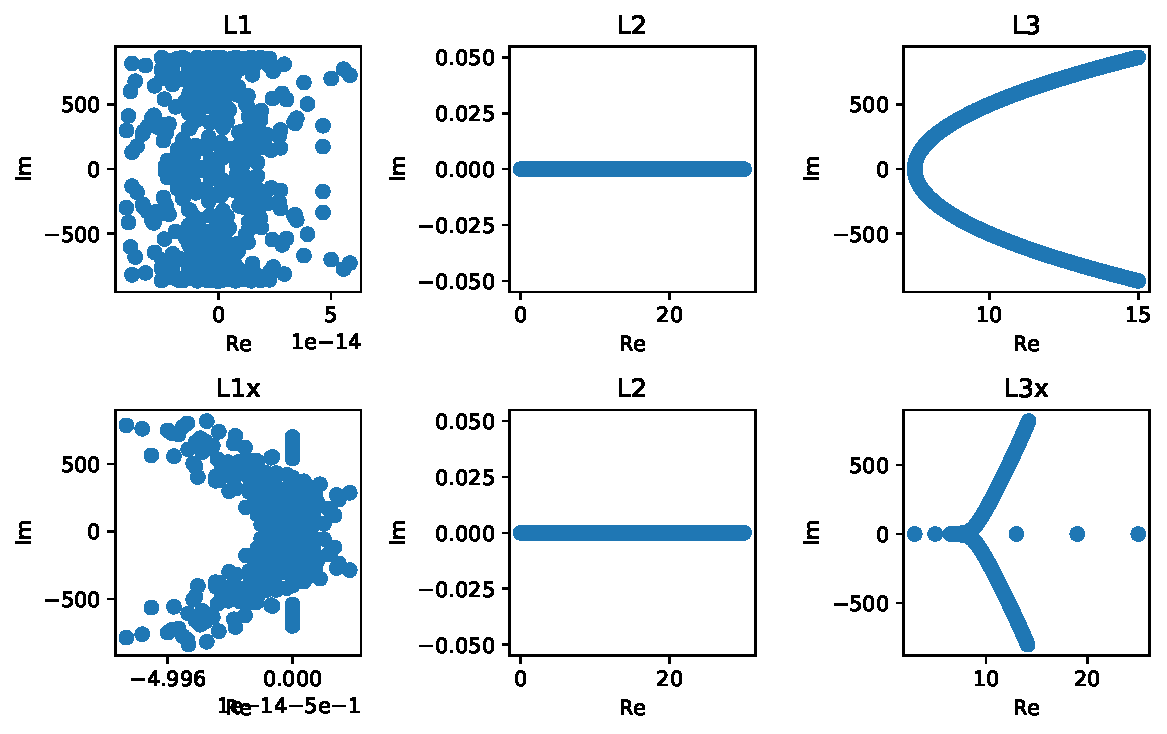
\includegraphics[width=0.8\textwidth]{eigs.pdf}
        \caption{Eigenvalues for the operators $L_1$, $L_2$, and $L_3$ with homogeneous Dirichlet conditions.\label{fig:eigenvalues}}
    \end{figure}
\end{solution}

\begin{exercise}{6.1}
    Show that the conditions in \cref{eq:6.15,eq:6.16,eq:6.17} are satisfied for $V_h = H^1_0$ and $Q_h = L^2$.
\end{exercise}

\begin{solution}{6.1}
    For this exercise we are considering Stokes problem, wherein we want to find $u_h \in V_h$ and $p_h \in Q_h$ such that
    \begin{equation}
        \begin{split}
            a(u_h, v_h) + b(p_h, v_h) &= f(v_h), \quad \forall v_h \in V_h, \\
            b(q_h, u_h) &= 0, \quad \forall q_h \in Q_h,
        \end{split}
    \end{equation}
    where
    \begin{equation}
        \begin{split}
            a(u, v) &= \int_{\Omega} \nabla u : \nabla v \diff x, \\
            b(p, v) &= \int_{\Omega} p \, \nabla \cdot v \diff x, \\
            f(v) &= \int_{\Omega} f \, v \diff x + \int_{\Omega_N} h \, v \diff s.
        \end{split}
    \end{equation}
    The conditions to show are then
    \begin{align}
        \text{\small Boundedness of $a$:}
        && \quad a(u_h, v_h) &\leq C_1 \norm{u_h}_{V_h} \norm{v_h}_{V_h},
        & \forall u_h, v_h \in V_h,
        \tag{6.15} \label{eq:6.15}
        \\
        \text{\small Boundedness of $b$:}
        && \quad b(q_h, u_h) &\leq C_2 \norm{q_h}_{Q_h} \norm{u_h}_{V_h},
        & \forall u_h \in V_h, q_h \in Q_h,
        \tag{6.16} \label{eq:6.16}
        \\
        \text{\small Coercivity of $a$:}
        && \quad a(u_h, u_h) &\geq C_3 \norm{u_h}_{V_h}^2,
        & \forall u_h \in Z_h,
        \tag{6.17} \label{eq:6.17}
    \end{align}
    where $Z_h = \{ u_h \in V_h \mid b(u_h, q_h) = 0, \, \forall q_h \in Q_h \}$.

    For \cref{eq:6.15}, we have
    \begin{equation}
        a(u_h, v_h) = \int_{\Omega} \nabla u_h : \nabla v_h \diff x,
    \end{equation}
    which by the Cauchy-Schwarz inequality is bounded by
    \begin{equation}
        a(u_h, v_h) \leq \norm{\nabla u_h}_{L^2} \norm{\nabla v_h}_{L^2} = \abs{u_h}_{H^1} \abs{v_h}_{H^1}.
    \end{equation}
    As we have previously shown that the $H^1$ semi-norm is equivalent to the $H^1$ norm, \cref{eq:6.15} is satisfied.

    For \cref{eq:6.16}, we have
    \begin{equation}
        b(q_h, u_h) = \int_{\Omega} q_h \, \nabla \cdot u_h \diff x,
    \end{equation}
    which by the Cauchy-Schwarz inequality is bounded by
    \begin{equation}
        b(q_h, u_h) \leq \norm{q_h}_{L^2} \norm{\nabla \cdot u_h}_{L^2}.
    \end{equation}
    We already have $\norm{q_h}_{L^2}$ as desired, and we now need to relate $\norm{\nabla \cdot u_h}_{L^2}$ to $\norm{\nabla u_h}_{L^2}$.
    We have
    \begin{align*}
        \abs{\nabla \cdot u(x)}^2
        &= \abs*{\sum_{i = 0}^{d} \frac{\partial u_i}{\partial x_i}(x)}^2
        \leq \left(
            \sum_{i = 0}^{d} 1
        \right) \left(
            \sum_{i = 0}^{d} \left( \frac{\partial u_i}{\partial x_i}(x) \right)^2
        \right)
        = d \sum_{i = 0}^{d} \left( \frac{\partial u_i}{\partial x_i}(x) \right)^2.
    \end{align*}
    Therefore,
    \begin{align*}
        \norm{\nabla \cdot u_h}_{L^2}^2
        &= \int_{\Omega} \abs{\nabla \cdot u_h}^2 \diff x
        \leq d \int_{\Omega} \sum_{i = 0}^{d} \left(
            \frac{\partial u_i}{\partial x_i}
        \right)^2 \diff x \\
        &\leq d \int_{\Omega} \sum_{i = 0}^{d} \sum_{j = 0}^{d} \left(
            \frac{\partial u_i}{\partial x_j}
        \right)^2 \diff x
        = d \int_{\Omega} \abs{\nabla u_h}^2 \diff x \\
        &= d \norm{\nabla u_h}_{L^2}^2.
    \end{align*}
    Using this, we have
    \begin{equation}
        b(q_h, u_h) \leq \sqrt{d} \norm{q_h}_{L^2} \norm{\nabla u_h}_{L^2},
    \end{equation}
    and as such \cref{eq:6.16} is satisfied.

    For \cref{eq:6.17}, we have
    \begin{equation}
        a(u_h, u_h)
        = \int_{\Omega} \nabla u_h : \nabla u_h \diff x
        = \norm{\nabla u_h}_{L^2}^2 = \abs{u_h}_{H^1}^2.
    \end{equation}
    As we have previously shown that the $H^1$ semi-norm is equivalent to the $H^1$ norm, \cref{eq:6.17} is satisfied.

    We have thus shown that the conditions in \cref{eq:6.15,eq:6.16,eq:6.17} are satisfied for $V_h = H^1_0$ and $Q_h = L^2$.
\end{solution}